% This is samplepaper.tex, a sample chapter demonstrating the
% LLNCS macro package for Springer Computer Science proceedings;
% Version 2.20 of 2017/10/04
%
\documentclass[runningheads]{llncs}
%
\usepackage{graphicx}
\usepackage{tikz}
\usepackage{pgfplots}
\pgfplotsset{compat=1.17}

%\usepackage{amsmath,amsthm,amsfonts,amssymb,latexsym}
\usepackage{amsmath,amsfonts,amssymb,latexsym}
% Used for displaying a sample figure. If possible, figure files should
% be included in EPS format.
%
% If you use the hyperref package, please uncomment the following line
% to display URLs in blue roman font according to Springer's eBook style:
% \renewcommand\UrlFont{\color{blue}\rmfamily}

\begin{document}
%
\title{Optimizacion de distribucion de antenas de telecomunicaciones}
%
%\titlerunning{Abbreviated paper title}
% If the paper title is too long for the running head, you can set
% an abbreviated paper title here
%
\author{Integrantes:\\ Carlos Garcia y Sebastian Pinzon \\
	\textbf{Entrega 1:Primera aproximaci\'{o}n del Modelo Matem\'{a}tico  \\Modelado, Simulaci\'{o}n y Optimizaci\'{o}n} \\}
%
%\authorrunning{F. Author et al.}
% First names are abbreviated in the running head.
% If there are more than two authors, 'et al.' is used.
%
\institute{Departamento de Ingenier\'{i}a de Sistemas y Computaci\'{o}n \\
	Universidad de Los Andes\\
	Bogot\'{a}, Colombia}
%
\maketitle              % typeset the header of the contribution
%
%
%
%
%\\
%Nombre:\\
\section{Descripci\'{o}n del Problema (30\%)}
En el mundo de las telecomunicaciones mantener conectados a los ususarios en la prioridad numero 1, sin embargo la infraestructura requiridad para esto puede llegar a ser muy costosa. Con esto en mente la optimizacion de la cobertura de las antenas usadas para conectar a los usuarios es muy importante. Las empresas tienen acceso a diferentes tipos de antenas con diferentes costos y diferents coberturas. Nuestro trabajo sera encontrar la manera de posicionar las antenas en un plano, maximizando cobertura y minimizando costos.
\\ \\
A pesar de que intentamos resolver un problema real, debemos tener en cuenta ciertas restricciones para la simplicidad del problema. Primero no tendremos en cuenta ni topologia ni logistica, en el mundo real hay contrucciones en ciertos lugares que no nos dejarian poner las antenas o caracteristicas geograficas que dificultan este proceso, como montañas o tereno inestable. Tambien tendros que ignorar aspectos tecnicos como interferencia de otras antenas. Sin embargo estas omiciones aun nos permiten extraer informacion valiosa para mejorar estos sistemas.
\\ \\
\begin{figure}
	\centering
	\includegraphics[width=0.3\textwidth]{plot3.png}
	\caption{Your Image Caption}
	\label{fig:your-image}
\end{figure}
\\



\begin{figure}[h]
	\begin{center}
		\centerline{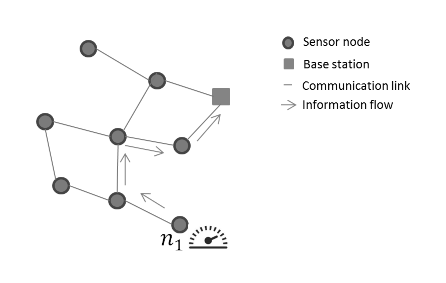
\includegraphics[scale=0.8]{./figures/network.eps}}
		\caption{Ejemplo de figura en Latex. \label{Fig:fig2}}
	\end{center}
\end{figure}


\section{Conjuntos, Par\'{a}metros y Variables (20\%)}

\textbf{*OBLIGATORIO: Describir por medio de tablas los conjuntos, par\'{a}metros y variables de decisi\'{o}n que se requieren para plantear el modelo matem\'{a}tico.}

\begin{table}[h]
	\caption{Conjuntos, Par\'{a}metros y Variables de decisi\'{o}n. \label{Tab: tab1}}
	\begin{tabular*}{\hsize}{@{\extracolsep{\fill}}ll@{}}
		\hline
		\textbf{Sets and Parameters} & \textbf{Description}\\
		\hline
		N &   Nodes set.\\
		S  & States set. \\
		$o$  & Source node.\\
		$d$  & Destination node.\\
		$st$  & State at which we want to obtain the minimum  \\
		& cost path from the \textit{Source} to the \textit{Destination}.\\
		$C_{it}^{jul}$ & Link cost from the node \textit{i} at the state \textit{t} to the \\ 
		& node \textit{j} at the state \textit{u} at the network state \textit{l}.\\
		\hline
	\end{tabular*}
\end{table}

% Table 1, part 2
\begin{table}[h]
	\caption{Variables de decisi\'{o}n}
	\begin{tabular*}{\hsize}{@{\extracolsep{\fill}}ll@{}}
		\hline
		\textbf{Variables} & \textbf{Description}\\
		\hline
		$X_{it}^{jul}$ &  Determines if the link at the state \textit{l} from the node \textit{i} at  \\ 
		&  the state \textit{t} to the node \textit{j} at the state \textit{u} is selected \\
		&  for building the path towards the \textit{Destination} (Binary variable). \\
		$Y_{i,l}$ &  Determines if the node \textit{i} at the state \textit{l} is selected as a \\
		&  forwarding node for building the path towards \\
		&  the \textit{Destination} (Binary variable).\\
		\hline
	\end{tabular*}
\end{table}

\newpage
\section{Funci\'{o}n Objetivo y Restricciones (50\%)}

\textbf{*OBLIGATORIO: Expresar matem\'{a}ticamente la funci\'{o}n objetivo (F.O) y las restricciones que delimiten el problema.}
\\ \\
\textbf{*OBLIGATORIO: Explicar en palabras la F.O y cada una de las restricciones teniendo en cuenta las delimitaciones del problema. En otras palabras, explicar el significado de cada restricci\'{o}n en el sentido de c\'{o}mo ayuda a solucionar o delimitar el problema.}
\\ \\
\textbf{*OBLIGATORIO: Tener en cuenta la mayor cantidad de limitaciones que pueda tener el problema. }

\begin{equation}
min (\sum_{i \in N} \sum_{j \in N} C_{ij} X_{ij})
\label{eq:res1}
\end{equation}

\begin{equation}
\sum_{j \in N} X_{ij} = 2   \qquad \forall{i \in N} \mid i=1
\label{eq:res2}
\end{equation}

\begin{equation}
 X_{ij} = 0   \qquad \forall{i \in N} \forall{i \in N} \mid i=j
 \label{eq:res3}
\end{equation}

La F.O indica que debemos tener en cuenta la...
\\
\\
La expresi\'{o}n \ref{eq:res2} representa el hecho de...
\\
\\
La expresi\'{o}n \ref{eq:res3} indica que debemos considerar la...

\textbf{Nota: si su proyecto requiere plantear varias F.O, describalas matem\'{a}ticamente as\'{i}:}
\begin{equation}
F.O 1: min (\sum_{i \in N} \sum_{j \in N} C_{ij} X_{ij}) 
\nonumber
\label{eq:res4}
\end{equation}

\begin{equation}
F.O 2: max (\sum_{i \in N} \sum_{j \in N} X_{ij})
\label{eq:res5}
\end{equation}


\section{Entregables}
\textbf{*OBLIGATORIO: El pdf con lo solicitado en el archivo "formatoYrequerimientosEntrega1.pdf".}
\\ \\
\textbf{*NOTA: NO hay que entregar ejecutables en GAMS o Pyomo. Esta primera entrega solo consiste en explicar el problema y proponer una primera aproximaci\'{o}n te\'{o}rica del modelo matem\'{a}tico.}


%
% ---- Bibliography ----
%
% BibTeX users should specify bibliography style 'splncs04'.
% References will then be sorted and formatted in the correct style.
%
% \bibliographystyle{splncs04}
% \bibliography{mybibliography}
%

\end{document}
